A second way in which the design of the site engenders accessibility can be seen from the screen shot within Figure \ref{fig:they-work-for-you-implementation-text-only-lynx}.
The screen shot depicts a terminal (or console) based text only browser, and it is displaying the information from the They Work for You site for the current UK Labour Party leader Jermey Corbyn.

\pagebreak
The text only browser displayed is called Lynx \cite{lynx}, which was created at the Univesity of Kanas in 1992, and which was successor to the first browser (known as 'WorldWideWeb' \cite{browser-history}) developed by Tim Bernes Lee \cite{tim-berners-lee}.

\begin{wrapfigure}{l}{0.50\textwidth}
  \centering
  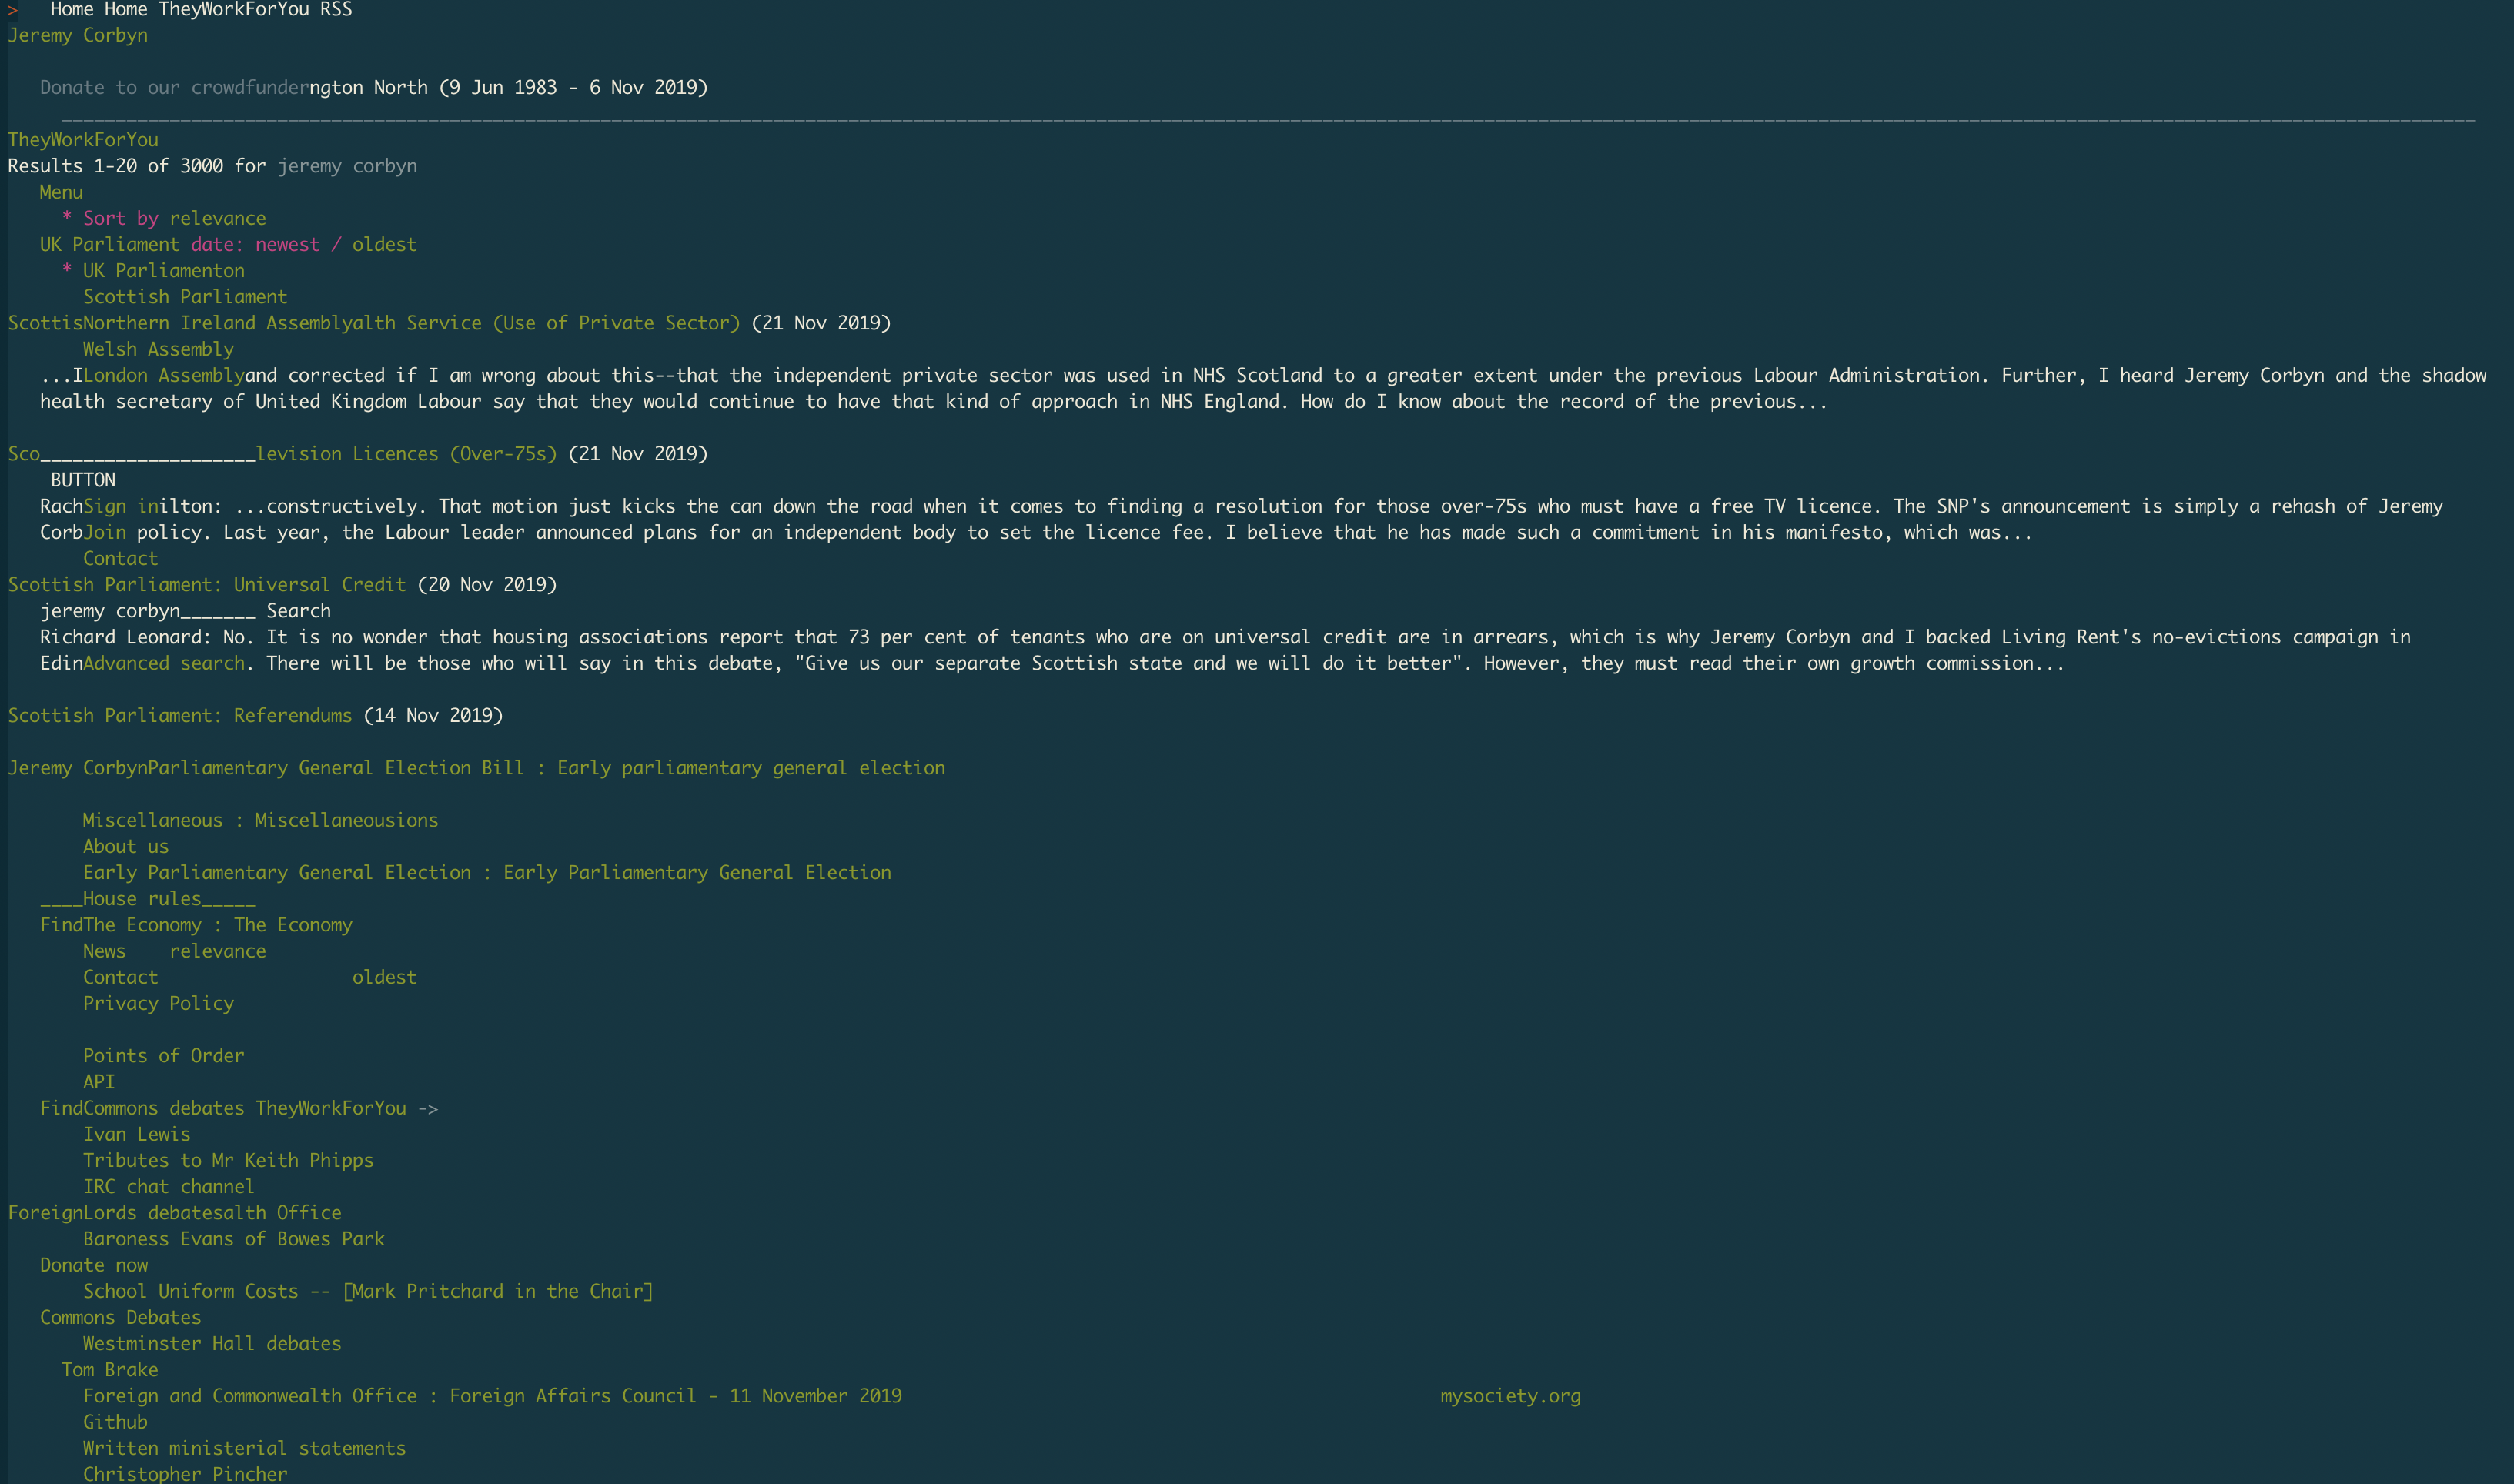
\includegraphics[scale=0.10]{images/they-work-for-you-implementation-text-only-lynx}
  \caption{Text only browsing via Lynx}
  \label{fig:they-work-for-you-implementation-text-only-lynx}
\end{wrapfigure}

Relatively few modern web sites fully support text only browsing, due to the inclusion of client side JavaScript DOM manipulation.
However, text browsers are frequently the basis for text to speech browsing (or transformations) as used by those with disabilities, such as blindness.
As such, the fact that the site can be viewed via a text only browser is another demonstration of how its design engenders accessibility, and, hence, contributes to civil society.
